\chapter{Beam profile}

\section{Slit experiment}
Figure \ref{fig:slit_photon} shows a photon, with two dimensions.
\begin{figure}[h!]
    \centering
    \includegraphics[width=0.35\textwidth]{slike/slit_photon.pdf}
    \caption{Photon}
    \label{fig:slit_photon}
\end{figure}
Heisenberg's uncertainty principle, equation \ref{eq:slt_hup}, shows that as the spatial distribution of EM waves
becomes more and more constrained the BPP must increase to preserve the minimum product.
\begin{equation}
    \Delta x \Delta p \ge \frac{h}{4 \pi}
    \label{eq:slt_hup}
\end{equation}

\section{Diffraction at a slit}
Diffraction of a monochromatic plane beam at a slit is shown in figure \ref{fig:slit1}.
\begin{figure}[h!]
    \centering
    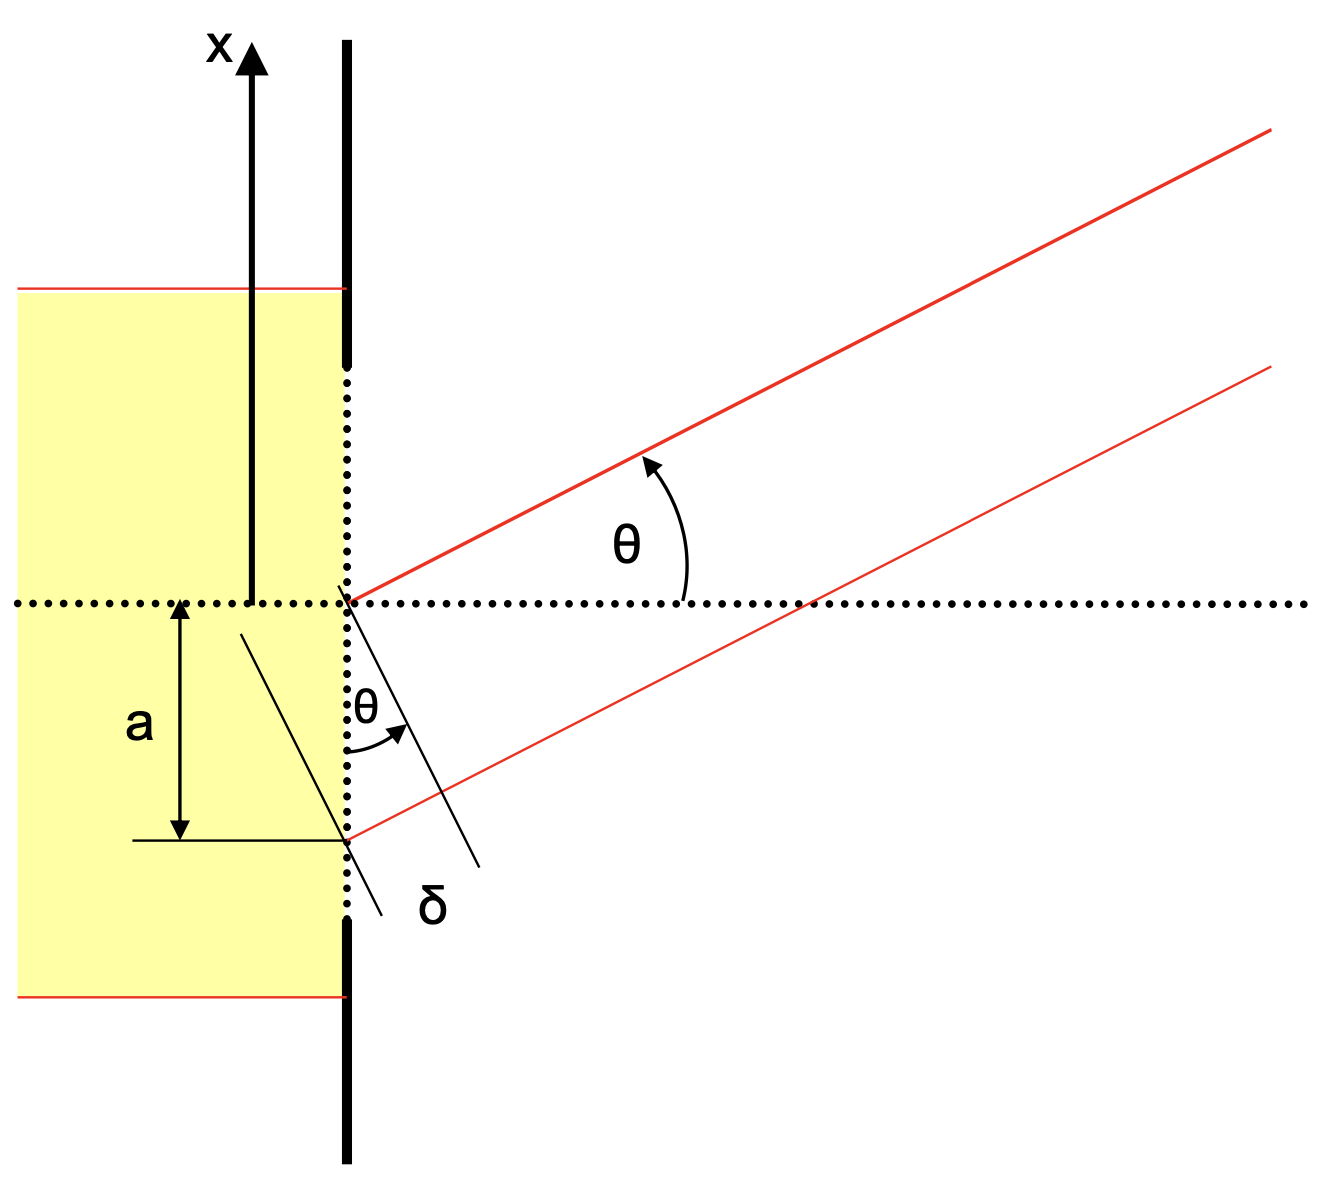
\includegraphics[width=0.35\textwidth]{slike/slit1.png}
    \caption{Diffraction at a slit}
    \label{fig:slit1}
\end{figure}
Another beam will have a path length difference of $\delta$, where $\delta = a \cdot sin(\theta)$, and a phase difference
of $\varphi = 2 \pi \frac{\delta}{\lambda} = \frac{2 \pi}{\lambda} \cdot a \cdot sin(\theta)$.
Sum of electric fields \ref{eq:sef}.
\begin{equation}
    \begin{aligned}
    E_{\sum} = E e^{i(k_z \cdot z + k_x \cdot x - \omega t)} + E e^{i(k_z \cdot z + k_x \cdot x - \omega t + \varphi)} =
    E e^{i(k_z \cdot z + k_x \cdot x - \omega t)} + E e^{i(k_z \cdot z + k_x \cdot x - \omega t + 2\pi \frac{\delta}{\lambda})} = \\
    E e^{i(k_z \cdot z + k_x \cdot x - \omega t)} + E e^{i(k_z \cdot z + k_x \cdot x - \omega t + \frac{2 \pi}{\lambda} \cdot a \cdot sin(\theta))} =  E_0(\vec{r},t) (1 + e^{i \frac{2\pi}{\lambda}a sin(\theta)}) 
    \end{aligned}
    \label{eq:sef}
\end{equation}

Interference for many beams, can be written as \ref{eq:imbd}.
\begin{equation}
    E_{\sum} = E_0(\vec{r},t) + \sum_{k=1,2,3...} E_0(\vec{r},t) e^{i\frac{2\pi}{\lambda}a_k sin(\theta)} =\sum_{k} E_0(\vec{r},t) e^{i\frac{2\pi}{\lambda}a_k sin(\theta)}
    \label{eq:imbd}
\end{equation}

For infinitely many beams the sum transitions to integration, as show in in equation \ref{eq:imb}.
\begin{equation}
    E_{\sum}(\vec{r},t) = \int_{-a_{max}}^{+a_{max}} E_0(\vec{r},t) e^{i\frac{2\pi}{\lambda} x sin(\theta)} dx
    \label{eq:imb}
\end{equation}
where $k_x(\theta) = \frac{2\pi}{\lambda} sin(\theta) = k_0 sin(\theta)$ and $E_0(\vec{r},t) = E e^{i(k_0 \cdot cos(\theta) \cdot z + k_0 \cdot sin(\theta) - \omega t)}$,
we can rewrite $E e^{i(k_0 \cdot cos(\theta) \cdot z + k_0 \cdot sin(\theta) - \omega t)} = E(\vec{r},t) e^{i(\frac{2\pi}{\lambda}x sin(\theta))}$ which is equal to
$E e^{i(k_0 \cdot cos(\theta) \cdot z - \omega \cdot t)} e^{i \cdot k_x(\theta) \cdot x}$. Combined we get the equation \ref{eq:fts}.
\begin{equation}
    E_{\sum} (\vec{r},t, \theta) = \int_{-a_{max}}^{+a_{max}} E_0(\vec{r},t) e^{i\cdot k_x(\theta) \cdot x} dx
    \label{eq:fts}
\end{equation}
We get symmetric \textbf{Fourier transform}. Table \ref{tab:ftp} shows the properties of the Fourier and inverse 
Fourier transform.
\begin{table}[h!]
    \begin{tabular}{|l|l|}
        \hline
        Forward transformation & Inverse transformation \\
        \hline
        time domain $\rightarrow$ frequency domain & time domain $\leftarrow$ frequency domain\\
        spatial domain $\rightarrow$ spatial frequency (angles) &spatial domain $\leftarrow$ spatial frequency\\
        $\hat{x}(\omega) = \mathcal{F}(x(t)) = \frac{1}{\sqrt{2\pi}} \int_{-\inf}^{\inf}x(t)e^{-i\omega t}dt$& $x(t) = \mathcal{F}^{-1}(\hat{x}(\omega))
        = \frac{1}{\sqrt{2\pi}} \int_{-\inf}^{\inf} \hat{x}(\omega)e^{i\omega t} d\omega$\\
        \hline
    \end{tabular}
    \caption{Properties of FT transform}
    \label{tab:ftp}
\end{table}

\subsection{Diffraction at rectangular aperture}
Intensity along $x$ axis is $I(\theta) = I_0 (sinc(\frac{A}{2} k sin(\theta)))^2$, with $sinc(x) = \frac{sin(x)}{x}$ 
and $k = \frac{2\pi}{\lambda}$($\pi$ phase shift), and $A$ the size of aperture.
Result of diffraction at a square aperture is shown on figure \ref{fig:squareaprture}.
\begin{figure}[h!]
    \centering
    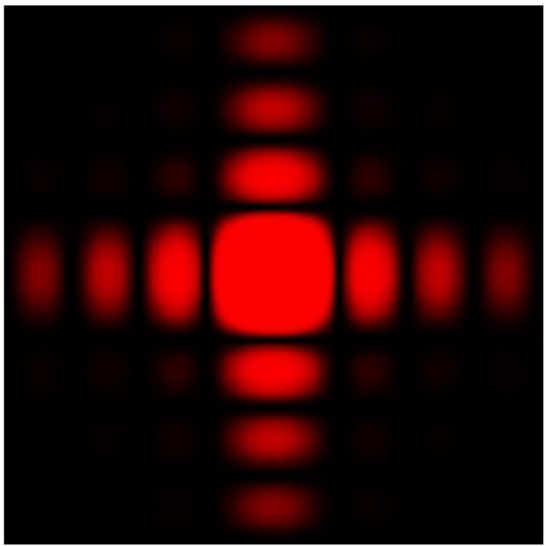
\includegraphics[width=0.15\textwidth]{slike/squareAdiff.png}
    \caption{Diffraction on square aperture. \sln}
    \label{fig:squareaprture}
\end{figure}

\subsection{Diffraction at round aperture}
Intensity along $x$ axis is given by \textit{Bessel J function} of the first kind $J_1(r)$. Equation \ref{eq:ira}
\begin{equation}
    I(\theta) = I_0 \left[\frac{2 J_1(\frac{A}{2} k sin(\theta))}{\frac{A}{2} k sin(\theta)}\right]^2
    \label{eq:ira}
\end{equation}
The lens allows us to observe at close distance, what we could see at the infinity. Figure \ref{fig:radf}.
\begin{figure}[h!]
    \centering
    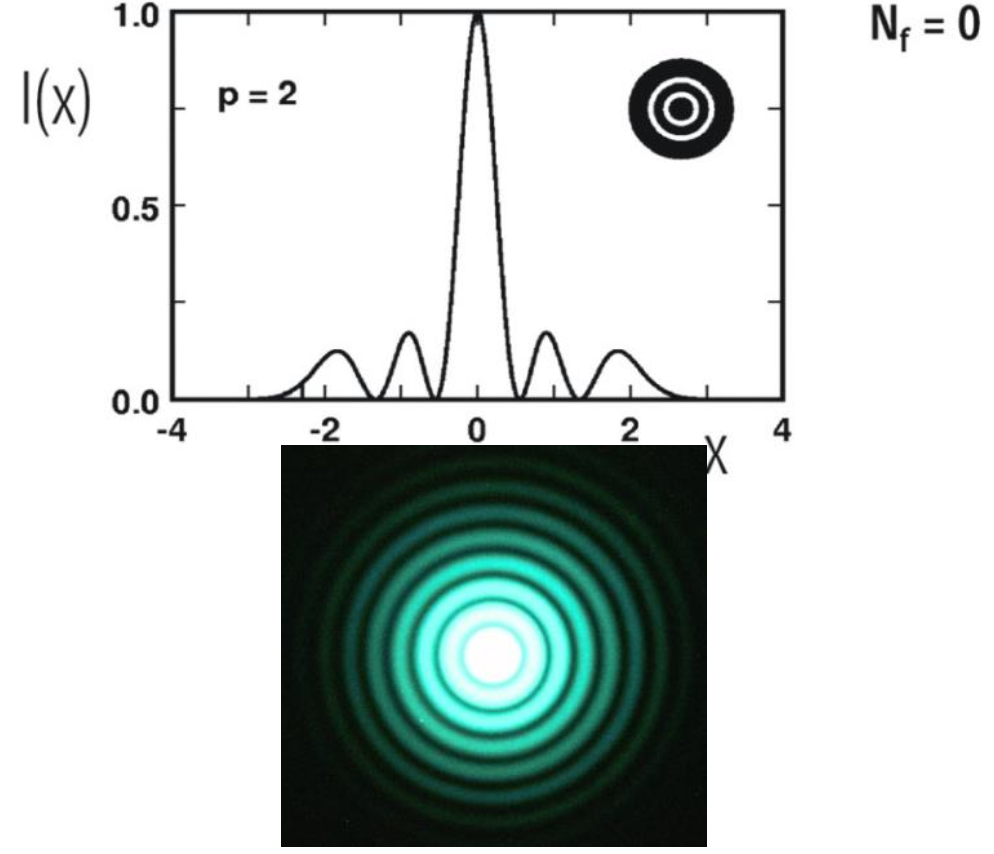
\includegraphics[width=0.25\textwidth]{slike/difSslt.png}
    \caption{Diffraction at round slit}
    \label{fig:radf}
\end{figure}

\subsection{Diffraction at resonator mirrors}
Diffraction on a mirror depends on mirror shape:
\begin{itemize}
    \item Plane mirrors - beam diffracts in the far field
    \item Concave mirrors - beam diffracts near the focal spot
\end{itemize}
In both cases, diffraction is given by the Fourier transform of mirror's aperture.
If beam intensity is homogeneous we have $sinc$ or $Bessel $ like diffraction patterns.

%333pp
\section{Fresnel number}
Fresnel number is a dimensionless number relating the pattern of beam light forms on a 
surface when projected through an aperture. Figure \ref{fig:fresnel1} shows the formation of the first minimum 
due to refraction on the first resonator mirror.

\begin{figure}[h!]
    \centering
    \includegraphics[width=0.5\textwidth]{slike/fresnel1.pdf}
    \caption{Formation of first minimum}
    \label{fig:fresnel1}
\end{figure}

Figure \ref{fig:fresnel2} show the reproduction of the maximum after one round trip in a resonator.
\begin{figure}[h!]
    \centering
    \includegraphics[width=0.5\textwidth]{slike/fresnel2.pdf}
    \caption{Two mirror resonator configuration}
    \label{fig:fresnel2}
\end{figure}

Accounting for $\Theta = \frac{\lambda}{2a}$ and $2 \cdot \Theta \le a$, we can derive \ref{eq:fres1}.
\begin{equation}
    \frac{L\lambda}{a} \le a
    \label{eq:fres1}
\end{equation}
And \ref{eq:fres2}, where $N_F$ is the \textbf{Fresnel number}.
\begin{equation}
    1 \le \frac{a^2}{L \lambda} = N_F
    \label{eq:fres2}
\end{equation}
$N_F = 1$ defines a length of $L=\frac{a^2}{\lambda}$ over which a plane of radius $a$ will propagate before developing strong diffracion rings.
If $N_F > 1$ the diffraction losses in resonator are minimal, if $N_F < 1$ losses in the resonator are high.
Fresnel number is related to distribution of intensity. Higher the Fresnel number, lower the losses.

\subsection{Intensity distribution}

Lower $N_F$ (e.g.:$N_F=1$) causes higher diffraction losses, beam quality and energy loss. Shown on figure \ref{fig:fbq1}.
 
\begin{figure}[h!]
    \centering
    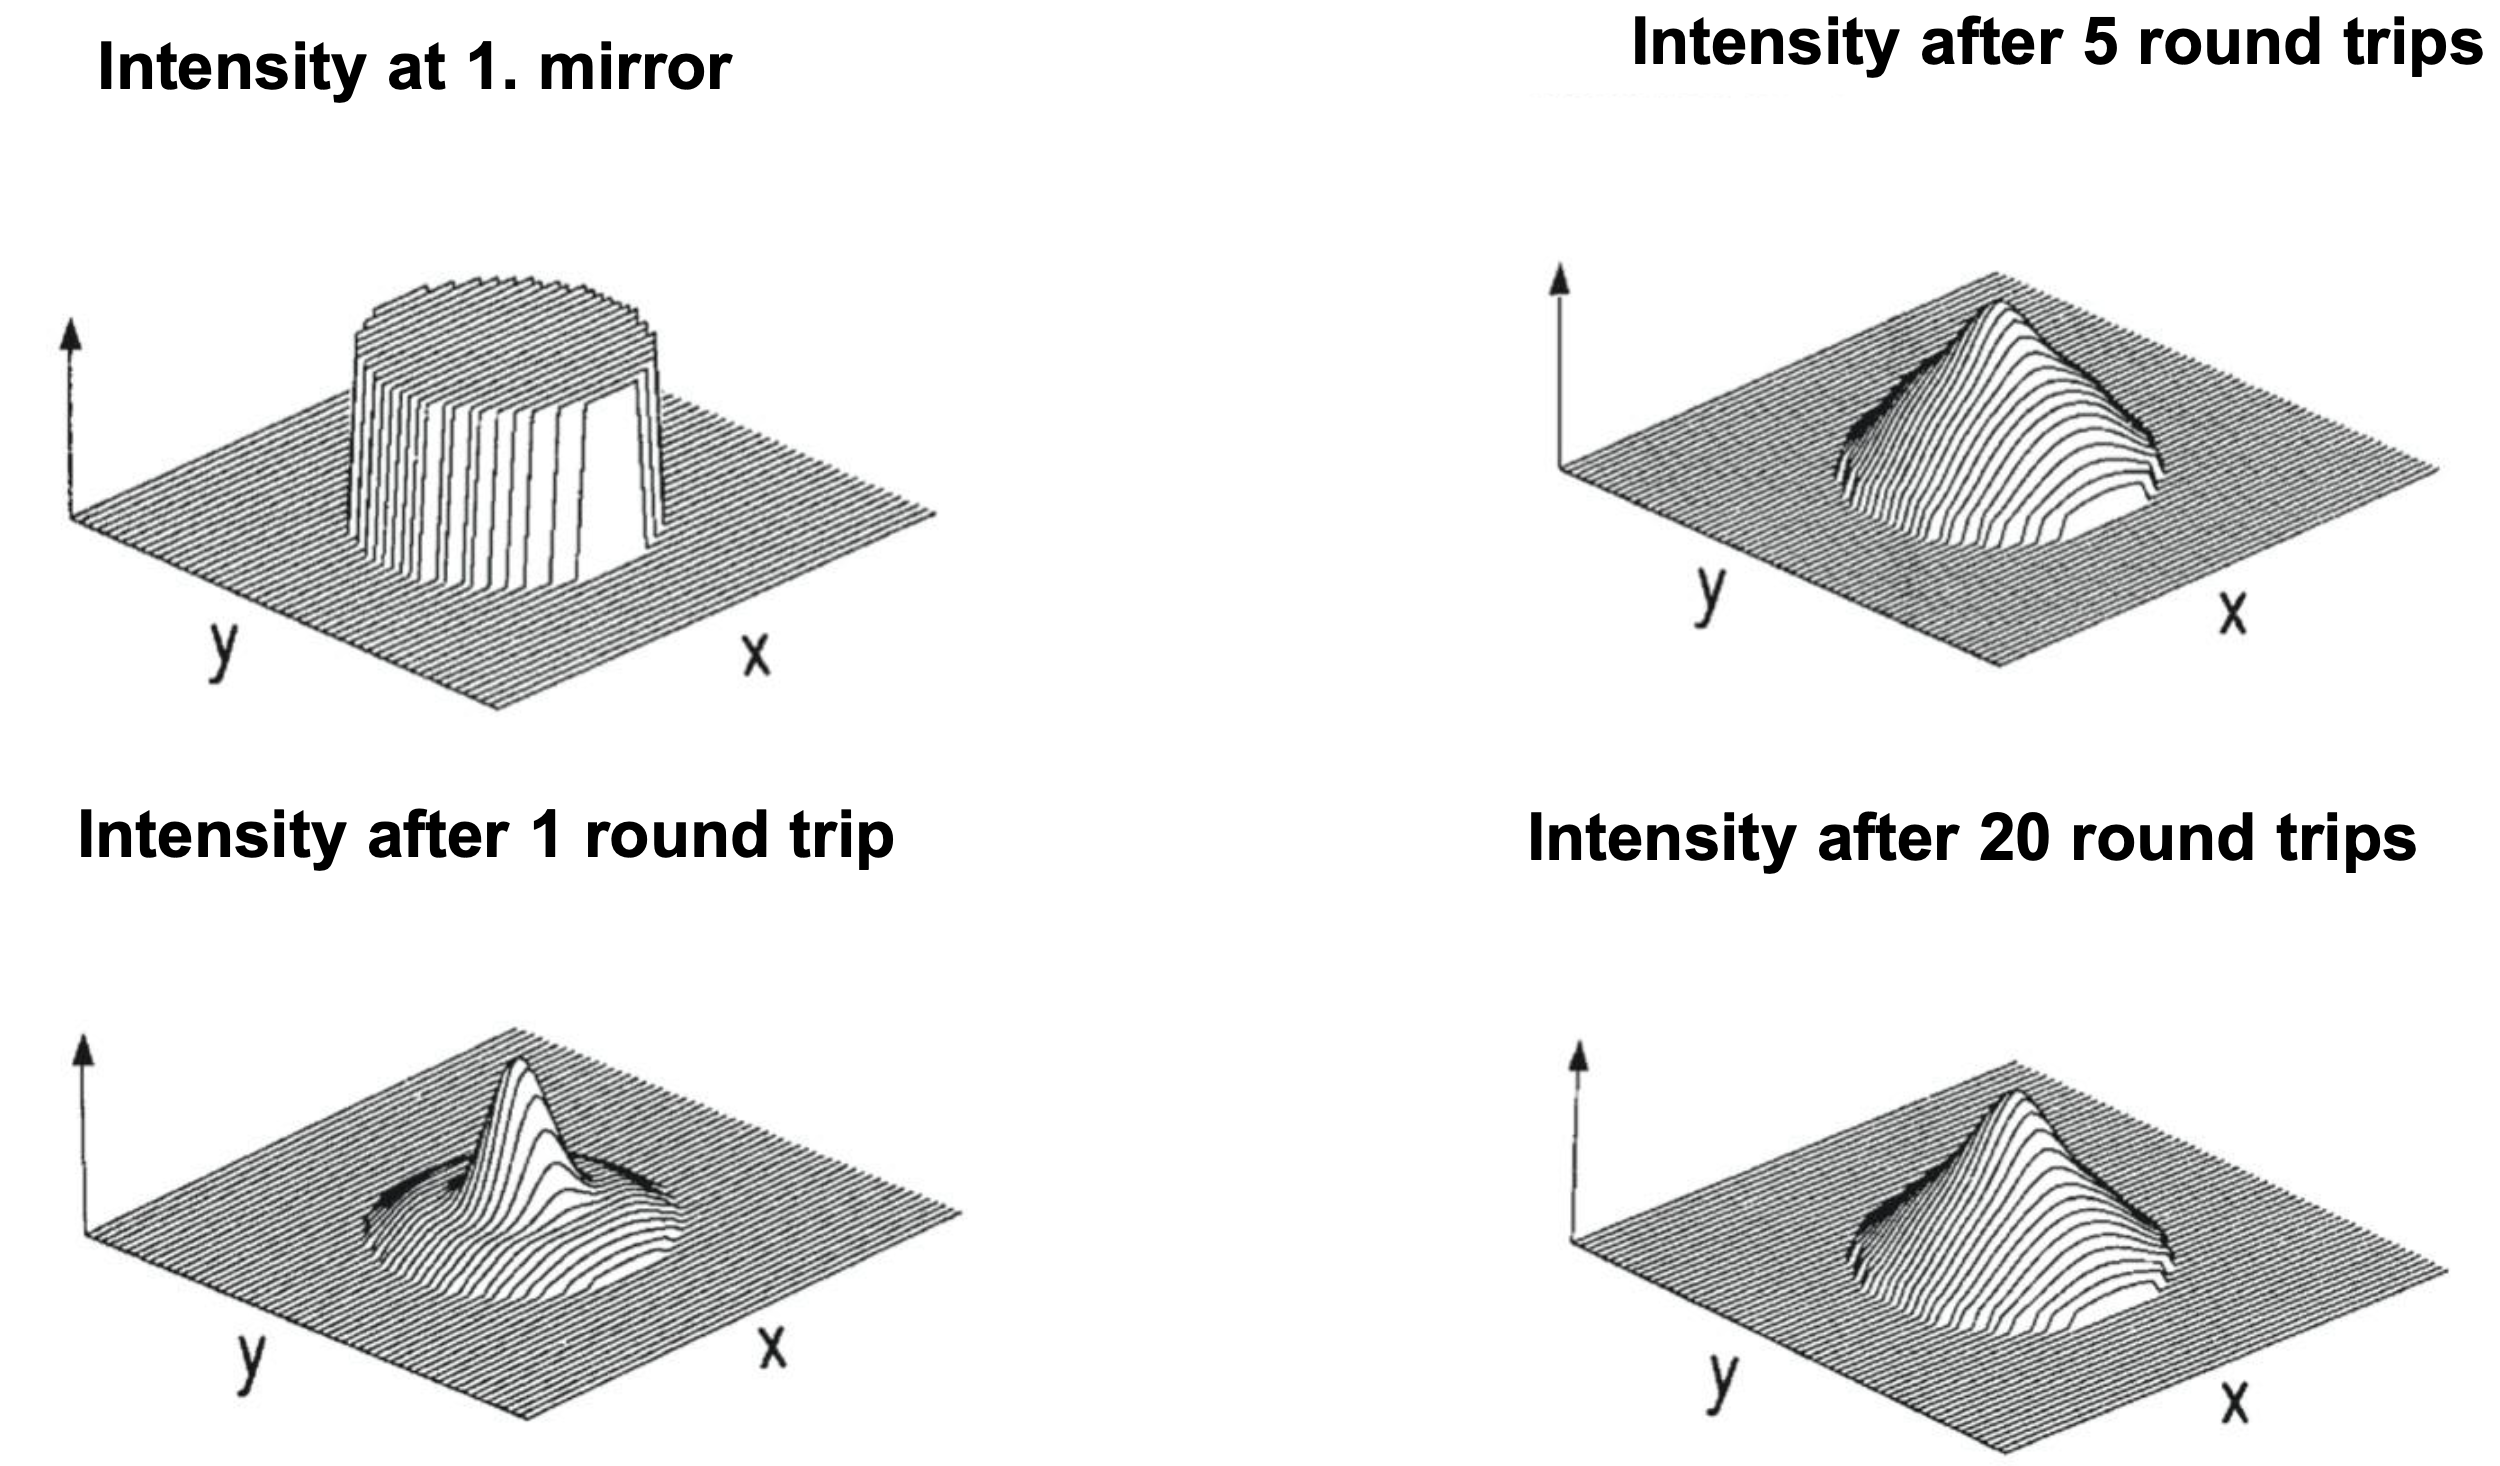
\includegraphics[width=0.5\textwidth]{slike/fbq1.png}
    \caption{Beam for $N_F=1$. \textit{Source:Lecture notes}}
    \label{fig:fbq1}
\end{figure}

A beam with $N_F=4$ has low diffraction losses and low improvement in beam quality - shown in figure \ref{fig:fbq2}.
\begin{figure}[h!]
    \centering
    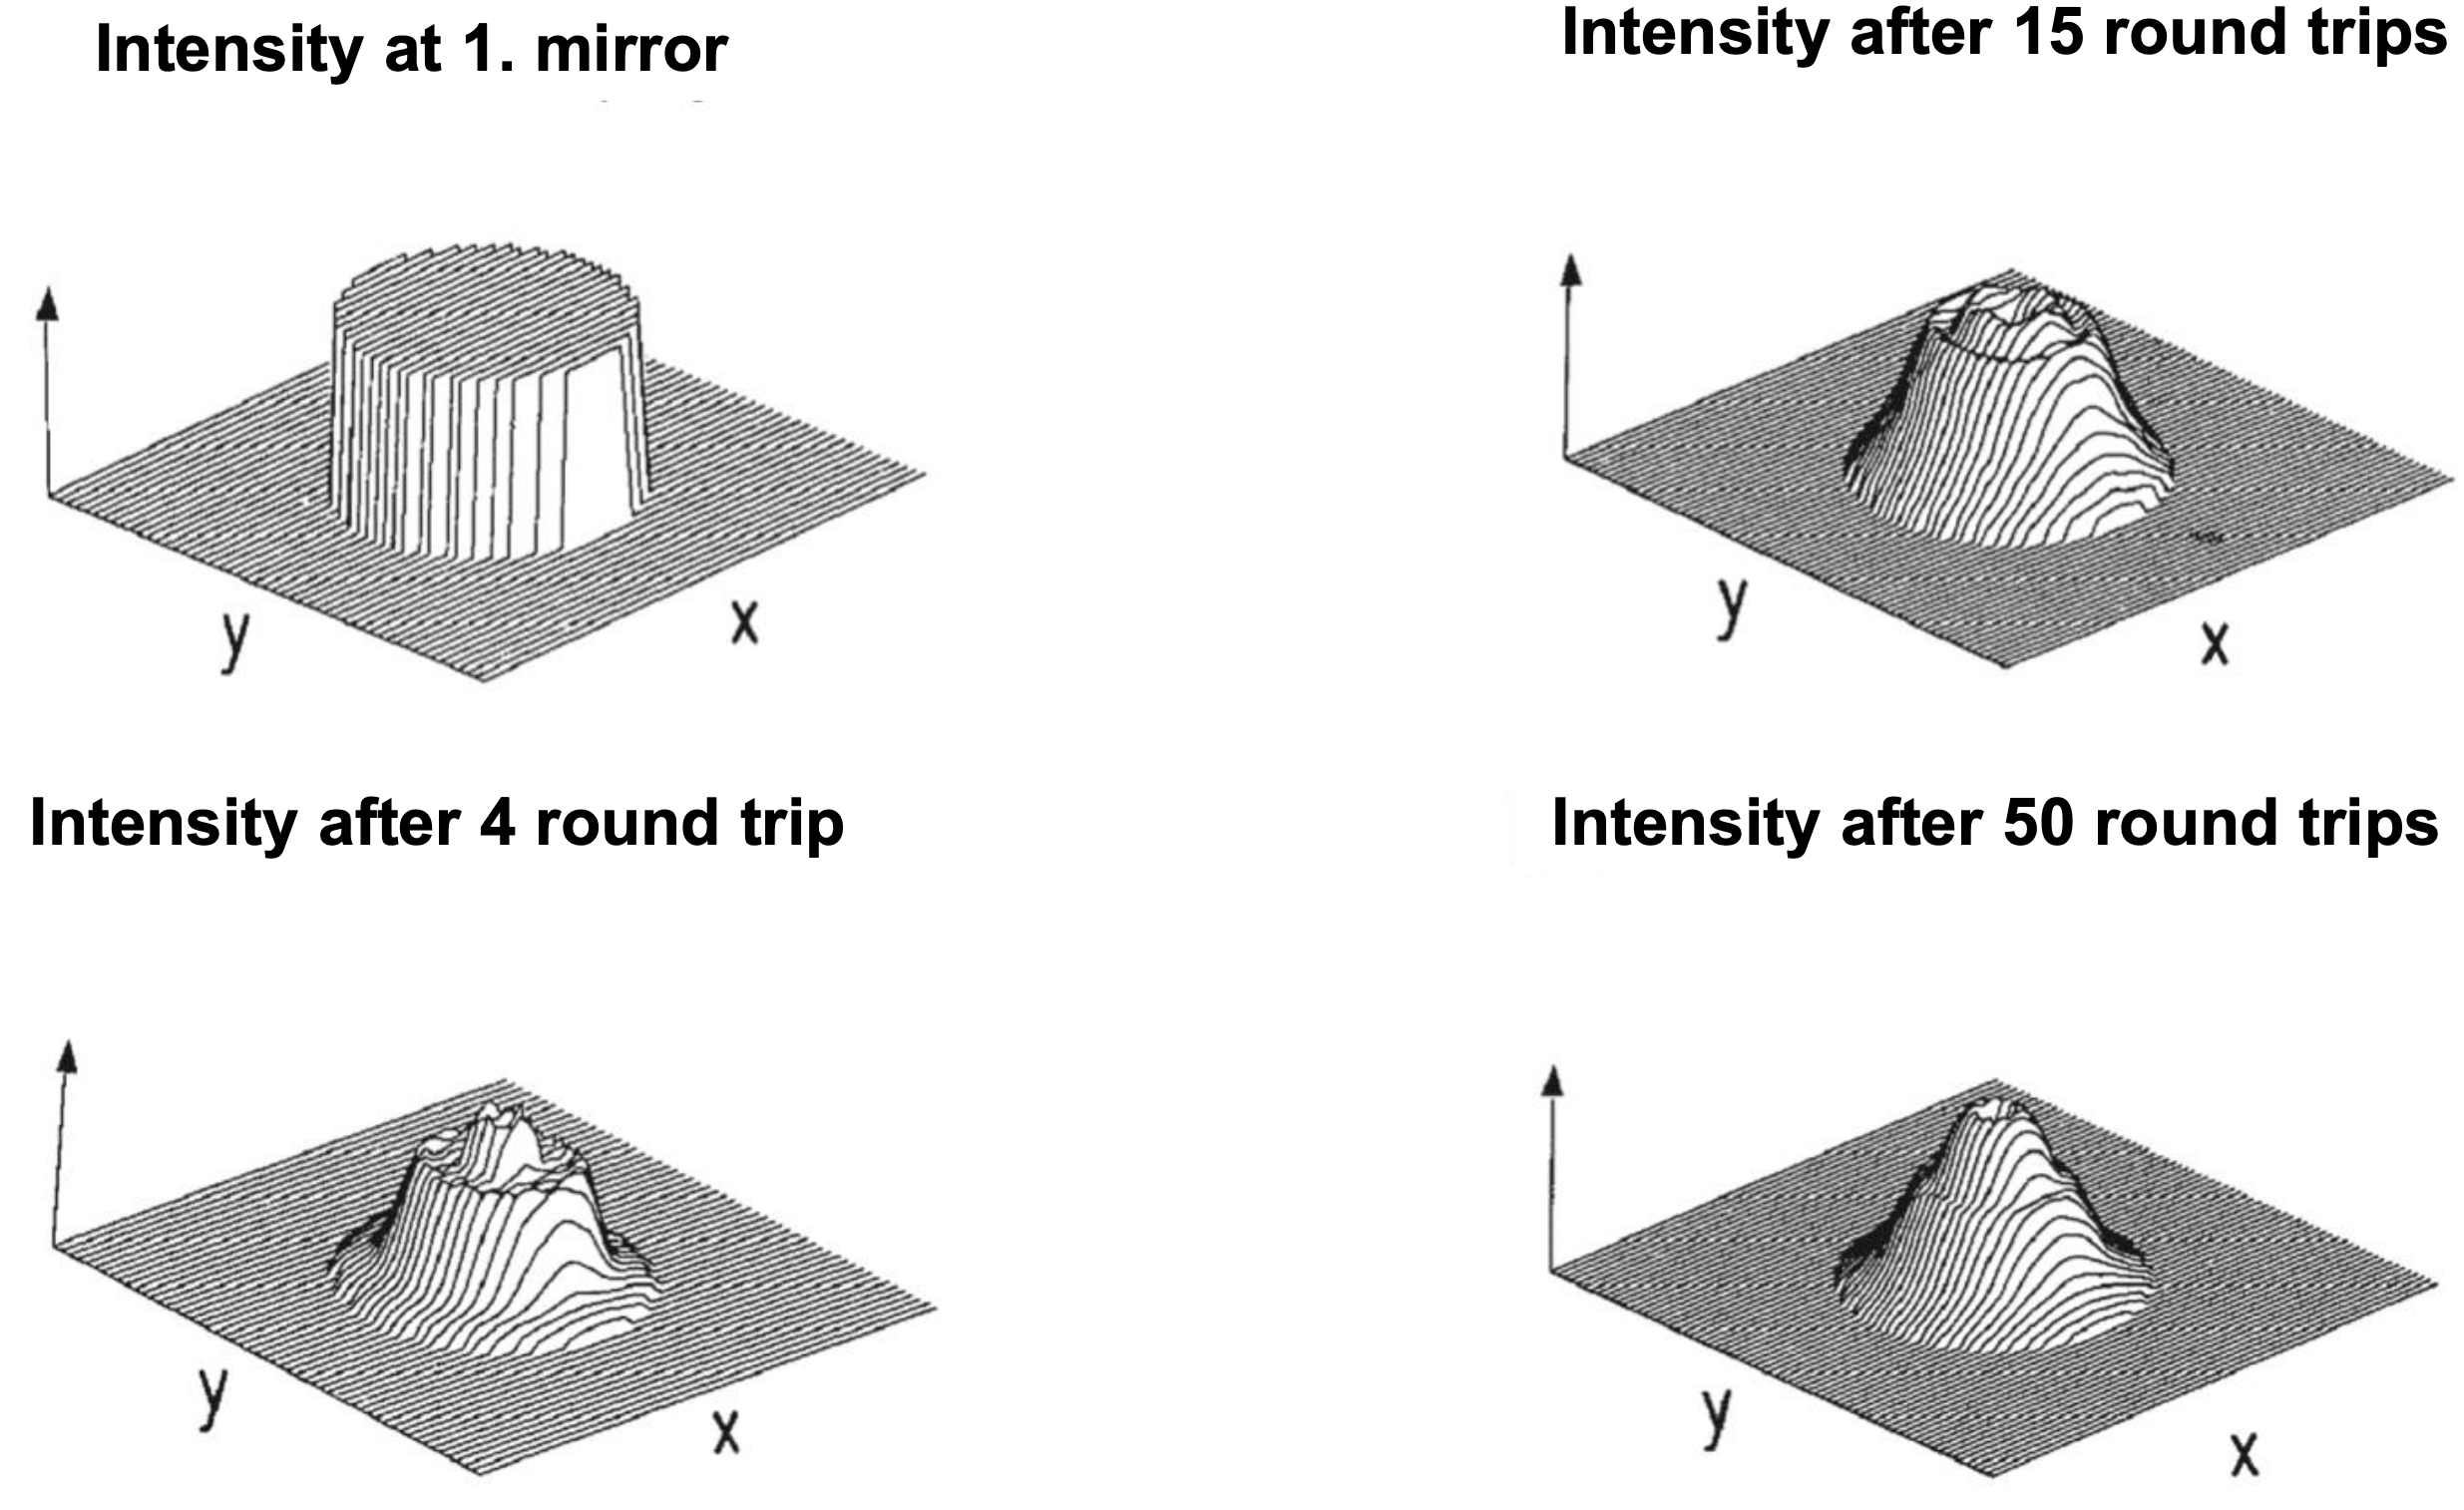
\includegraphics[width=0.5\textwidth]{slike/fbq4.png}
    \caption{Beam for $N_F=4$. \textit{Source:Lecture notes}}
    \label{fig:fbq2}
\end{figure}

\section{Multi Mode Operations}

In a stable resonator, stable beam trajectories satisfy the equation $R \cdot \vec{b} = \pm\vec{b}$.
Such beam must be an eigenstate of the resonator, in order to repeatedly pass through it. 

Laser active medium provides an intensity distribution $A_0 \cdot e^{-\frac{x^2}{2}}$.
Diffraction causes the profile to transform into a wave-vector distribution profile,
$\mathcal{F}(A_0 e^{-frac{x^2}{2}}) \rightarrow A_0 e^{-\frac{k^2}{2}}$, where $k$ is $x$ in angular space.

In the laser gain medium only certain waves gain energy, all waves loose energy due to
mirrors and other aperture-like components. (Main) Wave vector distribution is converted into
an intensity profile, equation \ref{eq:gdp1}.
\begin{equation}
    \mathcal{F} \left\{ A_0 e^{-\frac{k^2}{2}}\right\} \rightarrow A_0 e^{-\frac{x^2}{2}}
    \label{eq:gdp1}
\end{equation}
Such laser, with only one beam, has an EM-wave whose distribution is an eigenvector of a Fourier transform - equation \ref{eq:Item00}.
\begin{equation}
    I_{TEM_{00}} = I_0 exp \left( -2\frac{x^2+y^2}{w(z)^2}\right) = I_0 exp\left( -2 \frac{r^2}{w(z)^2} \right)
    \label{eq:Item00}
\end{equation}

\text{Such profile is called $TEM_{00}$}.

\subsection{Spatial hole burning}
When laser reaches population inversion in inhomogeneity, several \textbf{modes} can occur at the same time.

Figures $1.-4.$ shows the process of spatial hole burning. Population inversion is shown in picture $1.$,  Gaussian is excited first (picture $2.$) - centeral gain of the prifiles is reduced, but the 
outer area is mostly unused. In the population inversion in the outer area (picture $3.$) is high enough, the resonator can 
support more complex beam profile. Higher mode is excited (picture $4.$).

\begin{figure}[h!]
    \centering
    \includegraphics[width=0.65\textwidth]{slike/spatialholeburning.pdf}
    \caption{Spatial hole burning}
    \label{fig:shb}
\end{figure}
The spectral profile of new spectral shapes will not change as long as the new wavelength 
has the same losses and gain as the one before. 

\section{Transverse Electromagnetic Modes - TEM}
A \textbf{transverse mode} of electromagnetic radiation is an electromagnetic
field pattern of EM radiation in the plane perpendicular to the propagation direction.
Figure \ref{fig:tmpr} shows some possible modes in a passive resonator.
\begin{figure}[h!]
    \centering
    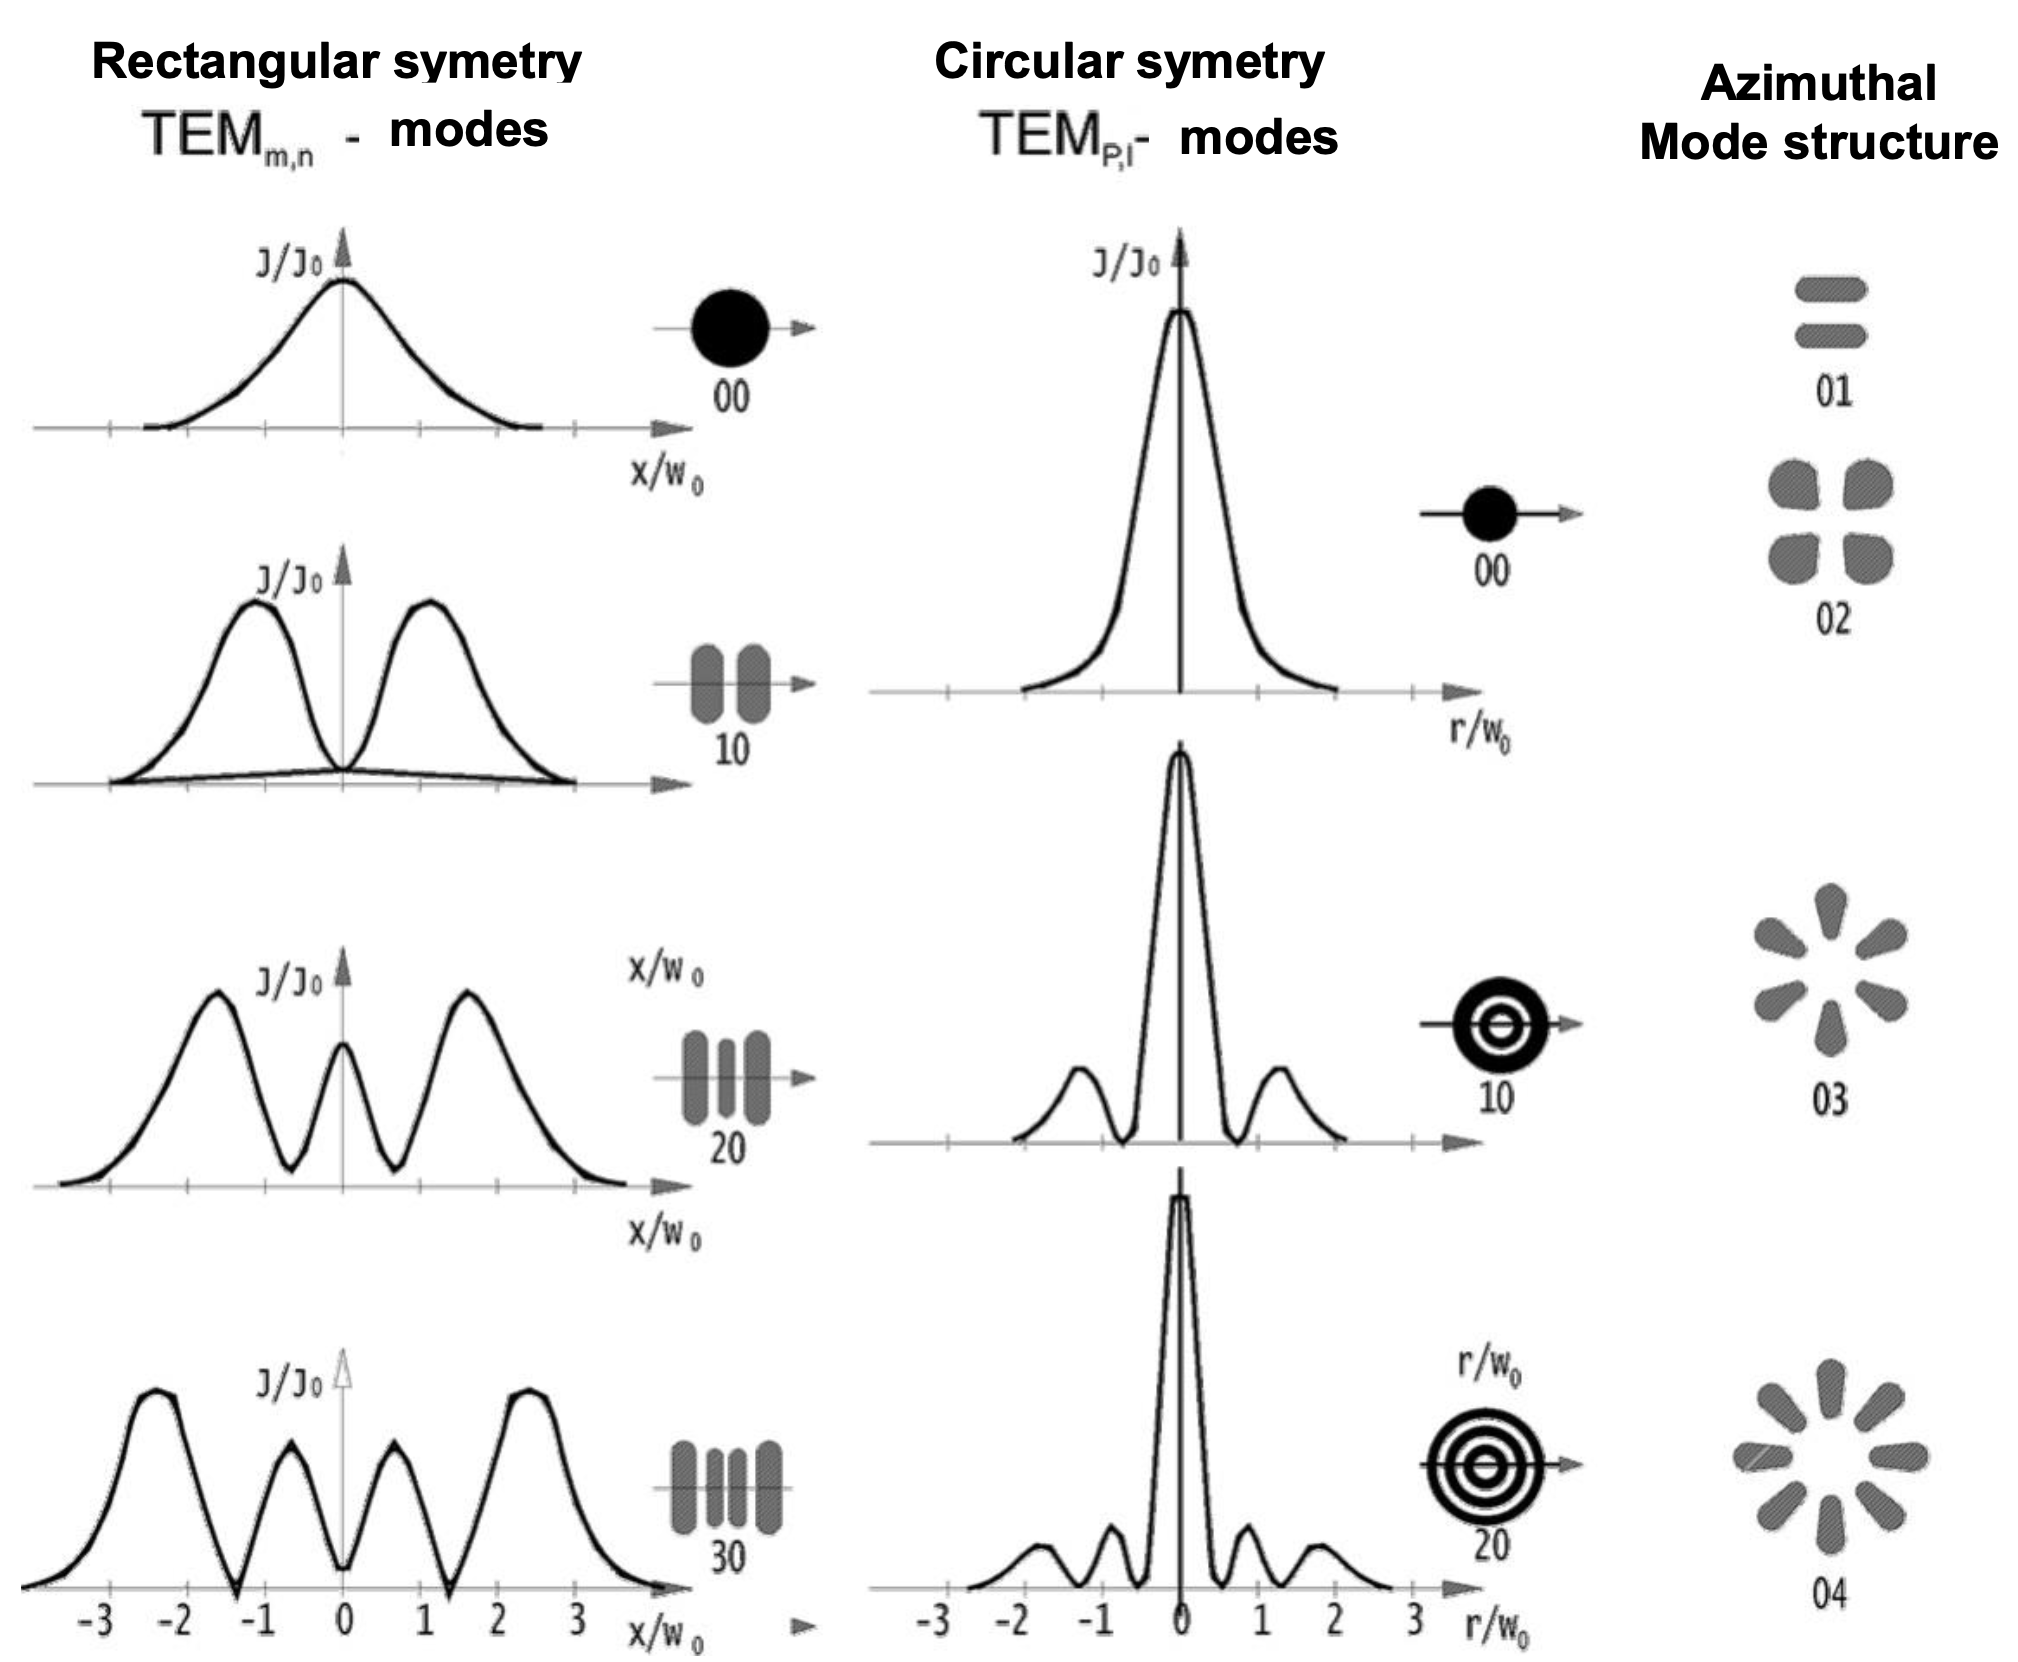
\includegraphics[width=0.5\textwidth]{slike/TransverseModes.png}
    \caption{Transverse modes of passive resonator.\\ \textit{Source: Lecture notes}}
    \label{fig:tmpr}
\end{figure}
Higher order $TEM$ can lead to complex polarization behaviour. In high power lasers several modes can overlap to create a hybrid mode.
If a laser emits more than one mode, it is called a multimode laser. A single mode laser emits mostly one or only one mode - $TEM_{00}$.
For applications that require good focusabillity we have to use a single mode laser.

Transverse modes are caused by path the light takes inside the resonator.
Actual path of the light ray is not equal to the distance between the mirrors. 


To reduce the amount of modes in a laser, we induce losses to higher order modes by placing a 
fixed or variable aperture inside the laser cavity.

\subsection{Circular symmetry}
In lasers, transverse modes are described as a combination of a \textbf{Gaussian beam} profile 
and a \textbf{Lagrange polynomial}. Modes are written as $TEM_{p,l}$, equation \ref{eq:temdef}.

\begin{equation}
    E_{p,l, \varphi} = E(0,z) \cdot exp\left( -\frac{r^2}{w(z)^2} \right) \cdot \left(\frac{\sqrt{2}r}{w(z)}\right)^l \cdot L^l_p \left(\frac{2r^2}{w(z)^2} \right) \begin{cases}
        cos(l\varphi)\\
        sin(l\varphi)
    \end{cases}
    \label{eq:temdef}
\end{equation}

$L^p_l$ is the \textbf{Lagrange polynomial}, $p$ is the degree of polynomial (number of zero crossings in radial direction) and $l$ is the number of zero crossing in $\varphi$ direction. 
Beam radios is given by $w$.

Figure \ref{fig:tmcr} shows shapes of different TEM.
\begin{figure}[h!]
    \centering
    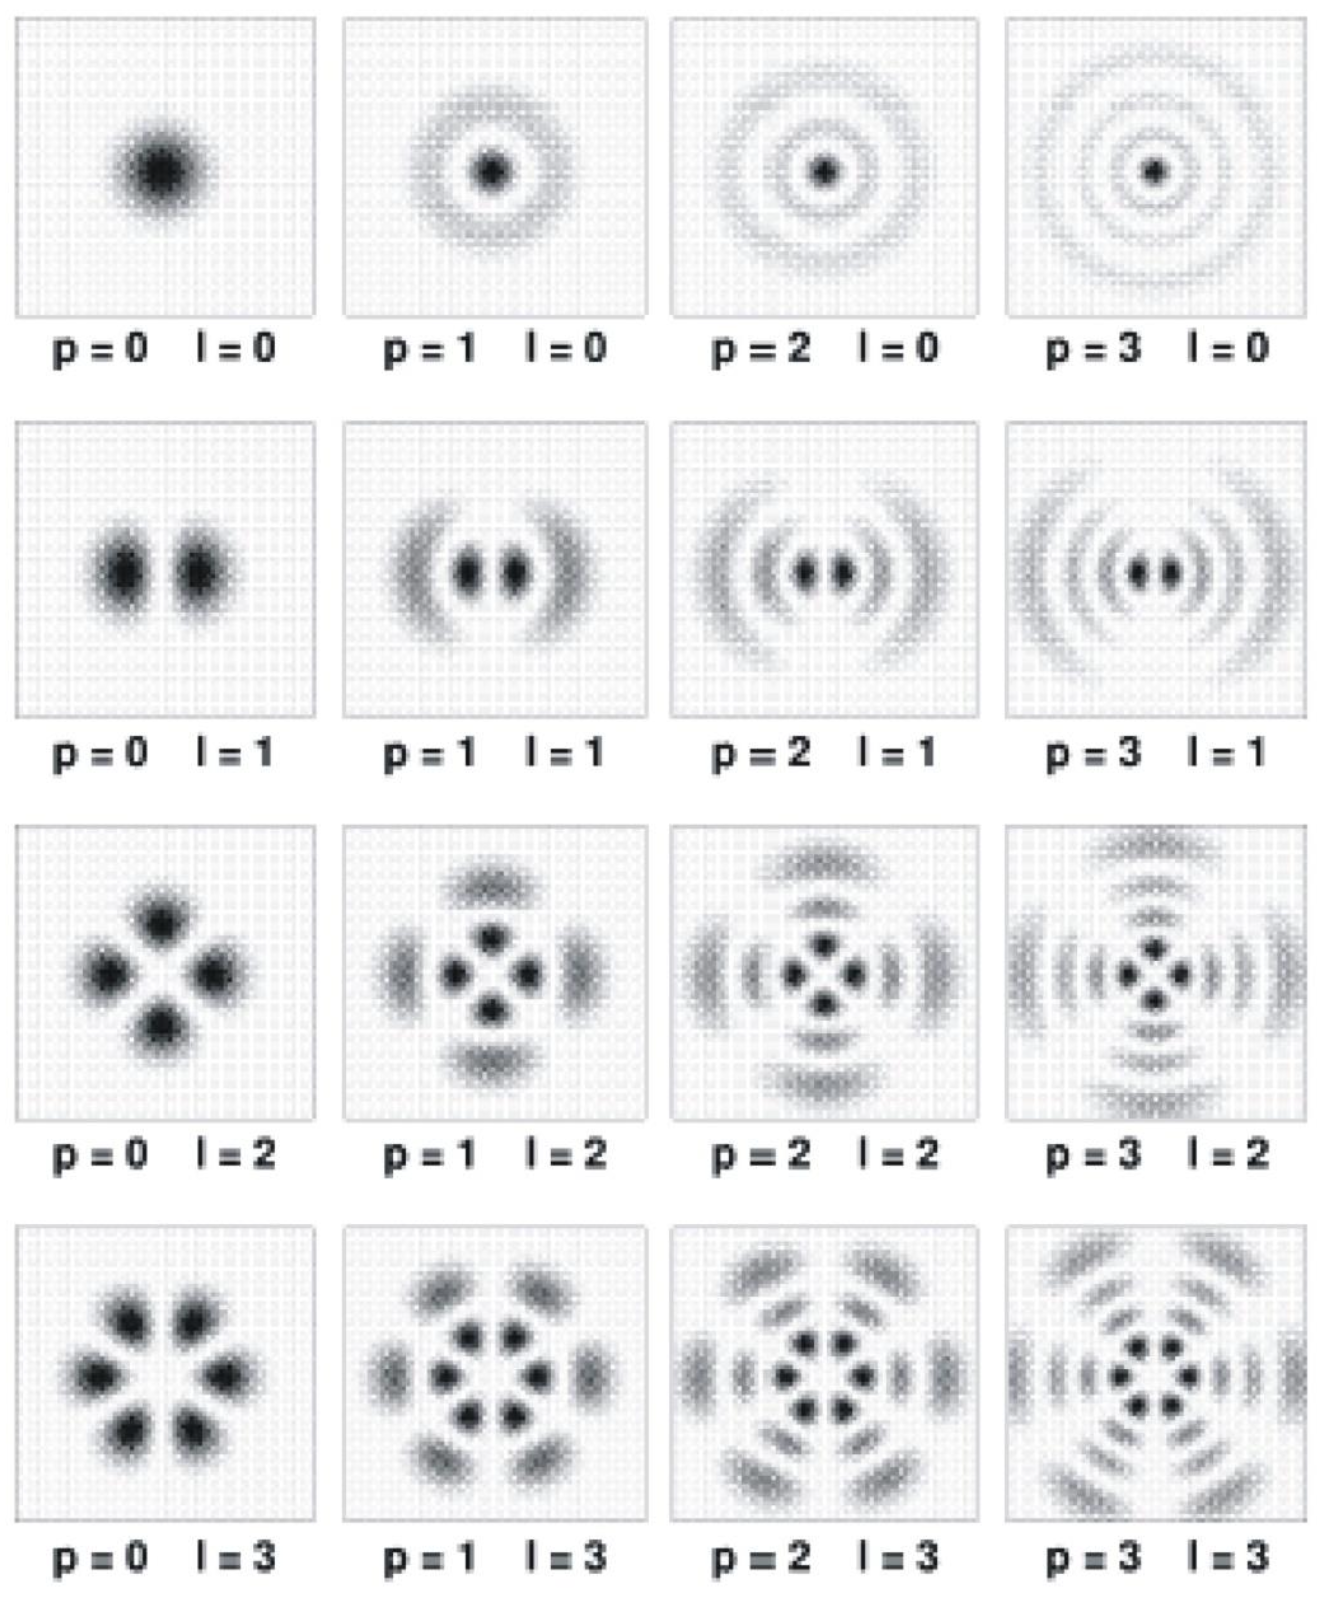
\includegraphics[width=0.3\textwidth]{slike/tmcr.png}
    \caption{Transverse mode structure in a circualr passive resonator.\\ \textit{Source: Lecture notes}}
    \label{fig:tmcr}
\end{figure}


\subsection{Rectangular symmetry}
%is profile equal to gauss and hermite polynomials.
For rectangular resonator symmetry, electric field is given by the equation \ref{eq:temrec}.
\begin{equation}
    E_{m,n} (x,y,z) = E(0,0,z) exp \left( -\frac{x^2+y^2}{w(z)^2} \right) \cdot H_m \left(\frac{\sqrt{2}x}{w(z)} \right) \cdot H_n \left(\frac{\sqrt{2}y}{w(z)} \right)
    \label{fig:temrec}
\end{equation}

Hermite polynomial $H_i$ has a degree - number of zero crossings - of $i$. Beam radius is equal to $w(z)$.
\begin{figure}[h!]
    \centering
    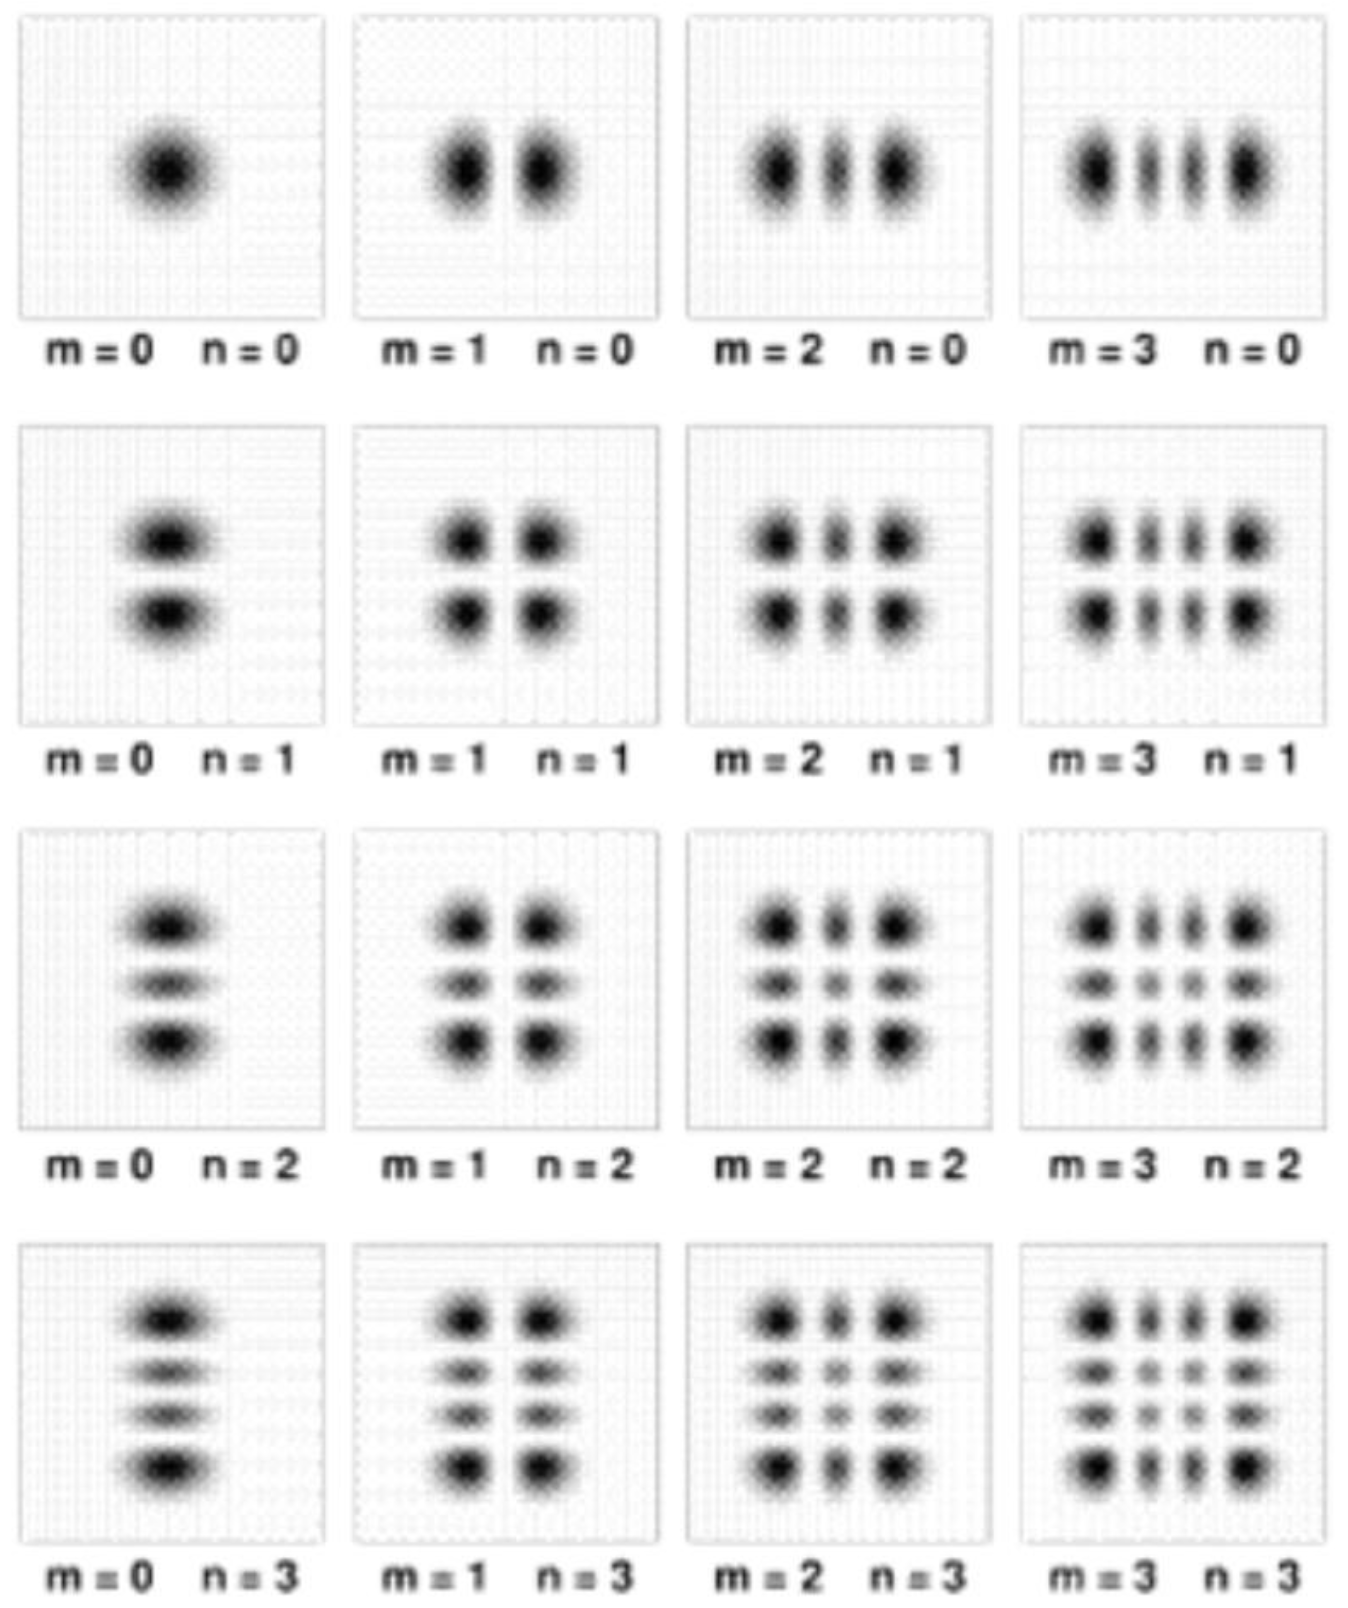
\includegraphics[width=0.3\textwidth]{slike/tmrr.png}
    \caption{Transverse mode structure in a rectangular passive resonator.\\ \textit{Source: Lecture notes}}
    \label{fig:tmrr}
\end{figure}



